\documentclass[11pt,a4paper]{article}

\usepackage{parskip,graphicx,fullpage,cmbright,wrapfig,url,fancyhdr}
\usepackage[T1]{fontenc}

\setlength{\headheight}{15.2pt}
\pagestyle{fancy}

\setlength{\topmargin}{-0.25in}

\lhead{Isabell Long}
\rhead{AS English Language \& Literature coursework}

\begin{document}

\title{An Excursion to York\ldots}
\author{Isabell Long}
\maketitle

Breathe a sigh of relief when you board the train at London King's Cross.  You're escaping!  After two hours, if the East Coast train's rear engine hasn't broken down, you'll hear the train guard announce ``the next station is York''.  Prepare to have a wonderful holiday!  

Presuming you arrive in the late afternoon, go and check into a \textbf{hotel}!  If you're looking for incredibly cheap options after the possibly bank-breaking train fare (though it's worth it, I promise), York has two Travelodges.  However, if you don't have friends or family to stay with and have come for a holiday, not a quick overnight work-related stay (if you haven't, why are you reading this article---go and be productive!), then treat yourself: if you want to go for expensive, the Cedar Court hotel and spa is extremely illustrious.  The luxurious Eygptian cotton bed linen on a King size bed and your own umbrella for the duration of your stay costs upwards of \pounds200 per night, which is to be expected, however, alternatively, The Royal York hotel is a short walk from the station and is more modestly priced with decent views of York's lovely Minster.

By far the trendiest mix of \textbf{restaurant and bar} is the Evil Eye Lounge on
Stonegate: the funky bar serving up a plethora of cocktails in the
evening, yet wonderful Thai food in the daytime up until around seven at
night.  Get in early, as it gets busy, and you wouldn't want to miss out
if you're into Thai spice---it's some of the best Thai food you will ever
taste in the UK, and the music choice is open so be prepared for some variation!  For something standard, especially useful if you're visiting with fussy kids, the usual array of pizza chains and caf\'es exist, but really, what's the fun in not exploring?  York boasts more than three hundred pubs, most relatively cheap and welcoming because they're northern, serving real ale from York's breweries, and even fruit wine!  The gentlemanly game hailing from Surrey, bar billiards, is still able to be played in the Waggon and Horses, though take a stopwatch---due to age and wear, the timing mechanism no longer functions.  If, on one night, you are craving some authentic Chinese food, Red Chilli restaurant, with its extensive menu, is the best sit down Chinese meal you will have unless you actually go to China.  The proof?  The food has made a Chinese person cry tears of joy.

York Minster is the biggest of York's \textbf{tourist attractions}.  Built between 1220 and 1470, it is York's cathedral that is adored by many and referred to as `the heart of Yorkshire'.  Christian worship still happens and there is no fee if you wish to go and participate in a service.  Walking to the top of the tower can be allowed for a fee, however ascending and descending 275 steps is definitely not for the faint-hearted!  If you would like to see the sights of York from above but aren't a climber, if you are not afraid of spinning wheels, York now has a London Eye equivalent on Station Road, though I'm not sure for how long, so hurry up your plans to visit.  It moves noticeably faster than the London attraction, so a good tip is to keep your eyes on the overall picture!

Born from the five year archeological dig that took place where the museum was subsequently built, the Jorvik Viking Museum enables its visitors to climb aboard time capsules and explore the city, smelling authentic aromas of home-cooked stew and seeing reconstructions of where the Vikings lived in 886AD.  All this costs only \pounds9.25 per adult and \pounds6.25 per child (above the age of five), with a \pounds26 deal for families of four.  Due to these prices and the sheer range of attractions, the queue can be hours long, so I recommend going at off-peak times.

\begin{wrapfigure}{l}{0.5\textwidth}
  \vspace{-10pt}
  \begin{center}
    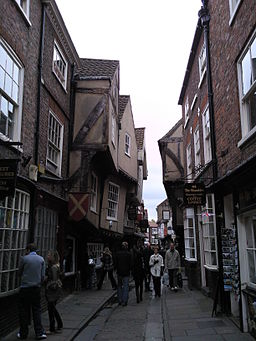
\includegraphics[width=0.50\textwidth]{shambles_overhangs_smaller}
  \end{center}
  \vspace{-20pt}
\end{wrapfigure}

\textbf{Do you or the kids fancy a gory, scary day?}  The York Dungeons
have a `fight to your death' gladiator attraction over Easter 2012, and the
constant possibility of travelling through some of York's bleak past.
You'll learn the story of Clifford's Tower, which you will then be able to
go and see.  York also boasts a `real' (over 700 year old) haunted house on
Stonegate, however due to steep stairs, it's not suitable for kids or
elderly people.  Not that I think they'd want to be scared out of their
wits!

Pick up a leaflet from the tourist information centre a short walk away from the station, and you'll get \pounds2 off entry fees, but for a limited time only.

The lack of mainstream \textbf{shopping} in York's centre is possibly quite surprising, however an attraction for the shoppers among you is the iconic, old-fashioned, cobbled, quirky street of the Shambles\footnotemark.  You'll laugh at the shops selling what the locals think of as tourist tat, such as dancing robotic cats, however you'll love the quirkier clothes shops and tea rooms---however none will beat the historic, iconic grand building and grand tea room Betty's in St. Helen's Square: people flock from miles around and queue for hours to sample delicious cakes and drinks.

York is a well-rounded city, with something for everyone.  Its \textbf{nightlife} is vibrant, as it must be, housing both the University of York and York St.\ John University.  The Mansion is a relatively newly branded nightclub on Micklegate, so you may still hear it referred to by its old name, Ziggy's.  It's not mainstream: it has more of a rock\slash metal\slash indie theme to it on Friday nights, which fits in well with its design.

\footnotetext{The image included in this document, the Shambles, was taken by `MuleAthon', is licensed under CC-BY-SA-3.0 (\url{www.creativecommons.org/licenses/by-sa/3.0}), and was sourced from Wikimedia Commons.}

All in all, you \textit{must} visit---York is an amazing city, and if I haven't convinced you by now, nothing will.  Now excuse me while I go and hop on a train\ldots you too?

\begin{center}
	\subsubsection*{Final word count (including footnotes): 1010 words.}
\end{center}

\end{document}
